\section{Umsetzung in KIV}

F�r die Umsetzung und Verifikation der Tiefensuche im KIV wurde die Graphenbibliothek von M. Drobek und D. Redlich verwendet (vgl. \cite{dr:2008}). Darauf aufbauend wurden zwei Spezifikationen entwickelt.
\par
\texttt{digraph-dfs-proc} spezifiziert die Tiefensuche, wie in Abschnitt \ref{sec:tiefensuche} beschrieben. Das bedeutet der R�ckgabewert ist entweder \texttt{true} oder \texttt{false}, abh�ngig davon, ob ein Knoten aus der Zielknotenmenge erreicht werden kann oder nicht. Eine genauere Beschreibung der Spezifikation erfolgt im Abschnitt \ref{sec:digraph-dfs-proc}.
\par
Dieser Spezifikation gen�gen die Module \texttt{dfs-it-1} als iterative Implementierung sowie \texttt{dfs-rek-1} als rekursive Implementierung. Details zu diesen Modulen k�nnen den Abschnitten \ref{sec:dfs-it-1} bzw. \ref{sec:dfs-rek-1} entnommen werden.
\par
Die zweite Spezifikation (\texttt{digraph-dfs-func}, vgl. Abs. \ref{sec:digraph-dfs-func}) definiert das Verhalten einer Variante der Tiefensuche, die zus�tzlich den Pfad vom Startknoten zu einem gefundenen Knoten aus der Zielknotenmenge liefert, sofern dieser existiert. F�r diese Spezifikation wurden ebenfalls eine rekursive (\texttt{dfs-rek-func}) und eine iterative Implementierung (\texttt{dfs-it-func-1}) umgesetzt. Genauere Beschreibungen zu diesen Modulen sind in den Abschnitten \ref{sec:dfs-rek-func} und \ref{sec:dfs-it-func-1} zu finden.
\par
Zus�tzlich wurde die Spezifikation \texttt{digraph-path} mit der zugeh�rigen Implementierung \texttt{dfs-temp} erstellt. Diese stellt einen Hilfssatz dar, der die Anzahl der erreichbaren Knoten von einem gegebenen Knoten (z.B. dem Startknoten) spezifiziert. Damit konnte eine Vereinfachung der Terminationsbeweise in den Modulen der Tiefensuche erreicht werden. Details dazu werden im Abschnitt \ref{sec:digraph-path} erl�utert.
\par
Zusammenfassend ist der komplette Projektgraph in Abb. \ref{fig:graph} dargestellt.

\begin{figure}[!htp]
	\centering
		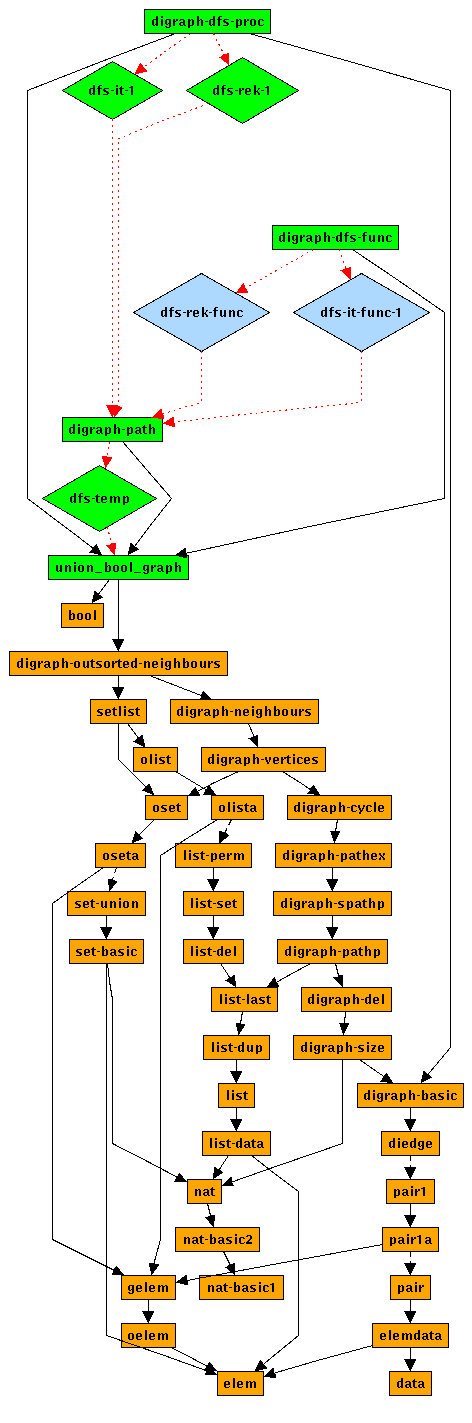
\includegraphics[height=0.7\paperheight]{img/graph.png}
	\caption{Projektgraph KIV}
	\label{fig:graph}
\end{figure}